\documentclass[11pt,a4paper]{article}
\usepackage[utf8]{inputenc}
\usepackage[T1]{fontenc}
% Rótulos em português (babel-brazilian indisponível neste ambiente de compilação;
% em TeX Live completo pode-se usar \usepackage[brazilian]{babel})
\renewcommand{\contentsname}{Sumário}
\renewcommand{\abstractname}{Resumo}
\renewcommand{\tablename}{Tabela}
\renewcommand{\figurename}{Figura}
\usepackage{amsmath,amssymb,bm}
\usepackage[margin=2.6cm]{geometry}
\usepackage{booktabs}
\usepackage{graphicx}
\usepackage[activate=false]{microtype}
\usepackage{xcolor}
\definecolor{linkblue}{RGB}{25,60,110}
\usepackage[colorlinks=true,linkcolor=linkblue,citecolor=linkblue,urlcolor=linkblue]{hyperref}
\usepackage{caption}
\captionsetup{font=small,labelfont=bf}
\usepackage{array}

\newcommand{\VaR}{\mathrm{VaR}}
\newcommand{\ES}{\mathrm{ES}}
\newcommand{\E}{\mathbb{E}}
\newcommand{\Prob}{\mathbb{P}}
\newcommand{\Ind}{\mathbb{I}}

\title{\textbf{CreditLens}\\[2mm]
\large Análise Quantitativa de Carteiras de Crédito:\\
Documentação Metodológica e Estudo de Caso}
\author{Walter C.~Neto\\[1mm]\small Baseado em D.~J.~Bolder, \emph{Credit-Risk Modelling} (Springer, 2018)}
\date{Julho de 2026 --- versão 0.5}

\begin{document}
\maketitle

\begin{abstract}
\noindent O \textbf{CreditLens} é um aplicativo de análise de risco de carteiras de crédito construído sobre as bibliotecas numéricas que acompanham o livro \emph{Credit-Risk Modelling: Theoretical Foundations, Diagnostic Tools, Practical Examples, and Numerical Recipes in Python}, de David Jamieson Bolder (Springer, 2018). A partir do upload de uma carteira em padrão CSV definido, o aplicativo estima a distribuição de perdas sob um portfólio de modelos --- independentes, \emph{mixture models}, \emph{threshold models} e o modelo regulatório (IRB de Basileia) ---, todos calibrados a um alvo comum de correlação de default. São reportados a perda esperada, a volatilidade da perda, o VaR e o \emph{Expected Shortfall} em múltiplos níveis de confiança, o capital regulatório com ajuste de granularidade e a decomposição do risco por contraparte. Este documento apresenta a arquitetura do aplicativo, o arcabouço teórico e matemático de cada modelo tal como implementado, e um estudo de caso completo sobre uma carteira hipotética de 250 contrapartes.
\end{abstract}

\tableofcontents

\section{O aplicativo}

O CreditLens opera em quatro etapas. Na \emph{ingestão}, o usuário carrega um arquivo CSV no padrão da ferramenta; o validador verifica a unicidade dos identificadores e os domínios das variáveis, aplica um piso regulatório de 3~pontos-base às PDs nulas e trunca os prazos ao intervalo $[1,5]$ anos exigido pelo ajuste de maturidade do IRB. Na \emph{calibração}, os parâmetros de dependência de cada família de modelos são ajustados a um mesmo alvo de correlação de default, o que torna as caudas diretamente comparáveis entre modelos. Na \emph{estimação}, todos os modelos são executados --- combinando fórmulas analíticas e simulação de Monte Carlo com $M$ trajetórias --- e, na \emph{apresentação}, os resultados são exibidos em tabelas e gráficos interativos, com exportação integral para Excel.

\subsection{Padrão de carteira}

Cada linha do arquivo CSV representa uma contraparte. As colunas obrigatórias são \texttt{id\_contraparte} (identificador único da contraparte), \texttt{exposicao} (o EAD, \emph{exposure at default} --- valor exposto no momento do default, estritamente positivo) e \texttt{pd} (probabilidade de default no horizonte de um ano, número em $(0,1)$). As colunas opcionais são \texttt{lgd} (\emph{loss given default} --- fração da exposição efetivamente perdida em caso de default, em $(0,1]$; valor-padrão $1{,}0$), \texttt{prazo\_anos} (prazo efetivo da operação, em anos, usado no ajuste de maturidade do IRB; valor-padrão $2{,}5$) e as colunas \texttt{rating} (funcional nos módulos de migração e ECL, em que mapeia a contraparte à linha da matriz de transição), \texttt{rating\_origem} (rating na originação, usado na classificação de estágios), \texttt{setor} (funcional no modelo multifatorial) e \texttt{nome} (descritiva). Seguindo a convenção de Bolder, toda a modelagem usa a \emph{severidade}
\begin{equation}
c_n = \mathrm{EAD}_n \times \mathrm{LGD}_n,
\end{equation}
em que $\mathrm{EAD}_n$ é a exposição da contraparte $n$ e $\mathrm{LGD}_n$ a sua perda dado o default; $c_n$ é, portanto, a exposição líquida sujeita a perda de cada contraparte, tratada como determinística ao longo de todo o documento.

\section{Arcabouço matemático}

\subsection{A perda da carteira}

Considere uma carteira com $N$ contrapartes, em que $p_n$ denota a probabilidade de default da contraparte $n$ e $c_n$ a sua severidade. Definindo o indicador de default $\Ind_{D_n}$, variável aleatória que vale $1$ se a contraparte $n$ entra em default no horizonte de um ano e $0$ caso contrário, a perda da carteira é
\begin{equation}
L \;=\; \sum_{n=1}^{N} c_n\,\Ind_{D_n}.
\label{eq:loss}
\end{equation}
O que distingue os modelos apresentados neste documento é, essencialmente, a estrutura de dependência imposta aos indicadores $\Ind_{D_n}$: é ela que governa a espessura da cauda de $L$ e, portanto, o capital econômico da carteira.

\subsection{Medidas de risco}

Para cada modelo, o CreditLens reporta quatro medidas. A \emph{perda esperada} é $\E[L]=\sum_n p_n c_n$. A \emph{volatilidade da perda} (ou perda não esperada, UL) é $\mathrm{UL}=\sqrt{\mathrm{Var}(L)}$. O \emph{valor em risco} no nível de confiança $\alpha$,
\begin{equation}
\VaR_\alpha(L) \;=\; \inf\{\ell : \Prob(L\le \ell)\ge\alpha\},
\end{equation}
é o menor valor de perda $\ell$ que não é excedido com probabilidade de pelo menos $\alpha$. O \emph{expected shortfall},
\begin{equation}
\ES_\alpha(L) \;=\; \E\!\left[L \mid L \ge \VaR_\alpha(L)\right],
\end{equation}
é a perda média nos cenários em que o VaR é atingido ou excedido --- por construção, $\ES_\alpha \ge \VaR_\alpha$. As medidas são calculadas nos níveis $\alpha\in\{95\%,\,99\%,\,99{,}9\%,\,99{,}97\%\}$. Nas implementações por Monte Carlo, elas são obtidas como estatísticas de ordem da distribuição simulada de $L$. O capital econômico usual é a parcela inesperada $\VaR_\alpha - \E[L]$.

\subsection{Índices de concentração}

O resumo da carteira inclui o índice de Herfindahl--Hirschman,
\begin{equation}
\mathrm{HHI}=\sum_{n=1}^N w_n^2, \qquad N_{\mathrm{efetivo}} = \mathrm{HHI}^{-1},
\end{equation}
em que $w_n = c_n/\sum_k c_k$ é a participação da contraparte $n$ na exposição líquida total. O inverso do HHI é o \emph{número efetivo de nomes}: quantas contrapartes de igual tamanho produziriam a mesma concentração. Esse indicador antecipa a magnitude do ajuste de granularidade da Seção~\ref{sec:irb}.

\section{O portfólio de modelos}

\subsection{Modelos independentes (cap.~2)}

O ponto de partida --- e contrafactual deliberadamente ingênuo --- assume defaults independentes entre contrapartes. Na versão analítica homogênea, toma-se $\bar p$ (a PD média da carteira ponderada por exposição) e a severidade média $\bar c$; o número de defaults $K$ segue então uma distribuição binomial,
\begin{equation}
\Prob(K=k)=\binom{N}{k}\,\bar p^{\,k}(1-\bar p)^{N-k},
\qquad
L \approx \bar c\,K,
\end{equation}
em que $k$ é o número de defaults observado e os quantis de $L$ são obtidos por interpolação da distribuição acumulada. Na versão de Monte Carlo heterogênea, sorteia-se para cada trajetória $m$ e contraparte $n$ um uniforme $U_{m,n}\sim\mathcal U(0,1)$ e declara-se default quando $U_{m,n}<p_n$, preservando a heterogeneidade de PDs e exposições. Pela lei dos grandes números, a independência elimina quase toda a variabilidade sistemática: a cauda resultante é fina demais para qualquer uso prudencial, e o papel do modelo aqui é servir de piso de referência para os demais.

\subsection{\emph{Mixture models} (cap.~3)}

Os \emph{mixture models} induzem dependência fazendo as PDs compartilharem um fator aleatório comum. Condicionalmente ao fator, os defaults são independentes; incondicionalmente, tornam-se correlacionados.

\paragraph{Beta-binomial.} A probabilidade comum de default é sorteada de $Z\sim\mathrm{Beta}(a,b)$, em que $a$ e $b$ são os parâmetros de forma da distribuição beta; dado o sorteio de $Z$, cada contraparte entra em default de forma independente com probabilidade $Z$. A calibração resolve o sistema
\begin{equation}
\E[Z]=\frac{a}{a+b}=\bar p,
\qquad
\rho_D=\frac{1}{a+b+1}=\rho_D^{\mathrm{alvo}},
\end{equation}
em que $\rho_D$ denota a correlação de default entre pares de contrapartes e $\rho_D^{\mathrm{alvo}}$ é o alvo escolhido pelo usuário. É o \emph{mixture model} mais parcimonioso e tende a produzir caudas pesadas quando $\rho_D^{\mathrm{alvo}}$ é alto em relação a $\bar p$.

\paragraph{CreditRisk\textsuperscript{+} (Poisson-gama, um fator).} O fator sistemático é $S\sim\Gamma(v,\,1/v)$, distribuição gama parametrizada de modo que $\E[S]=1$ e $\mathrm{Var}(S)=1/v$ --- ou seja, $v$ controla a volatilidade do ciclo: quanto menor $v$, mais volátil o fator. A intensidade condicional de default de cada contraparte é
\begin{equation}
p_n(S) = p_n\,\bigl(1-w+wS\bigr),
\end{equation}
em que $w\in(0,1)$ é a carga do fator, isto é, a fração da intensidade que responde ao ciclo (o complemento $1-w$ é a parcela idiossincrática). Os defaults são gerados por uma contagem de Poisson $H_n\sim\mathrm{Poisson}\bigl(p_n(S)\bigr)$, com default declarado quando $H_n\ge 1$. Trata-se do arcabouço atuarial clássico de portfólio de crédito, que reaparece na Seção~\ref{sec:irb} como base analítica do ajuste de granularidade.

\subsection{\emph{Threshold models} (cap.~4)}

Nos \emph{threshold models}, o default ocorre quando uma variável latente --- interpretada como o retorno dos ativos da contraparte --- cai abaixo de um limiar. Na família gaussiana de um fator, espinha dorsal da prática de mercado e do próprio IRB, o estado latente da contraparte $n$ é
\begin{equation}
Y_n \;=\; \sqrt{\rho}\;G \;+\; \sqrt{1-\rho}\;\varepsilon_n,
\qquad G,\varepsilon_1,\dots,\varepsilon_N \overset{iid}{\sim}\mathcal N(0,1),
\label{eq:threshold}
\end{equation}
em que $G$ é o fator sistemático comum a toda a carteira, $\varepsilon_n$ é o choque idiossincrático da contraparte $n$ e $\rho\in(0,1)$ é a correlação de \emph{ativos}, que dosa o peso do fator comum. O default ocorre quando $Y_n < \Phi^{-1}(p_n)$, sendo $\Phi^{-1}$ a inversa da distribuição normal-padrão acumulada --- o limiar é escolhido de modo que a probabilidade incondicional de default seja exatamente $p_n$. A correlação de \emph{default} implícita entre duas contrapartes com PDs $p$ e $q$ é
\begin{equation}
\rho_D(p,q;\rho) \;=\;
\frac{\Phi_2\!\bigl(\Phi^{-1}(p),\Phi^{-1}(q);\rho\bigr)-pq}
{\sqrt{p(1-p)}\sqrt{q(1-q)}},
\label{eq:rhoD}
\end{equation}
em que $\Phi_2(\cdot,\cdot;\rho)$ é a distribuição normal bivariada acumulada com correlação $\rho$ --- o numerador é a probabilidade de default conjunto menos o produto das marginais. O CreditLens calibra $\rho$ numericamente para que $\rho_D(\bar p,\bar p;\rho)$ iguale o alvo comum definido pelo usuário.

\paragraph{Variante t-Student.} Substituindo o vetor gaussiano por
\begin{equation}
Y_n=\sqrt{\tfrac{\nu}{V}}\Bigl(\sqrt{\rho}\,G+\sqrt{1-\rho}\,\varepsilon_n\Bigr),
\qquad V\sim\chi^2_\nu,
\end{equation}
em que $V$ é um choque radial qui-quadrado com $\nu$ graus de liberdade, comum a todas as contrapartes, e o limiar passa a ser $t_\nu^{-1}(p_n)$ (inversa da distribuição t de Student), o modelo adquire \emph{dependência de cauda}: mesmo mantida a correlação $\rho$, defaults conjuntos extremos tornam-se ordens de magnitude mais prováveis, porque um sorteio pequeno de $V$ amplifica simultaneamente todos os $Y_n$. Poucos graus de liberdade ($\nu$ baixo) engordam a cauda; no limite $\nu\to\infty$ recupera-se o caso gaussiano.

\paragraph{ASRF (carteira assintótica).} No limite de uma carteira infinitamente granular e homogênea, o modelo gaussiano admite a solução fechada de Vasicek:
\begin{equation}
\VaR_\alpha \;=\; \Bigl(\textstyle\sum_n c_n\Bigr)\;
\Phi\!\left(\frac{\Phi^{-1}(\bar p)+\sqrt{\rho}\,\Phi^{-1}(\alpha)}{\sqrt{1-\rho}}\right),
\label{eq:vasicek}
\end{equation}
em que $\sum_n c_n$ é a exposição líquida total, $\bar p$ a PD homogênea da carteira, $\rho$ a correlação de ativos e $\alpha$ o nível de confiança. É o esqueleto analítico do IRB e, neste documento, funciona também como verificação de consistência do modelo \emph{threshold} simulado.

\subsection{Capital regulatório IRB e ajuste de granularidade (cap.~6)}
\label{sec:irb}

O requerimento de capital do IRB, avaliado contraparte a contraparte, é a perda inesperada condicional ao cenário sistemático de 99{,}90\%, multiplicada pelo ajuste de maturidade:
\begin{equation}
K_n \;=\;
\Bigl[
\Phi\!\Bigl(\tfrac{\Phi^{-1}(p_n)+\sqrt{\rho_B(p_n)}\,\Phi^{-1}(0{,}999)}{\sqrt{1-\rho_B(p_n)}}\Bigr)
- p_n
\Bigr]\cdot \mathrm{MA}(M_n,p_n),
\qquad
\mathrm{Capital}=\sum_n c_n K_n,
\label{eq:irbK}
\end{equation}
em que $K_n$ é o coeficiente de capital da contraparte $n$ (fração da severidade $c_n$ exigida como capital), $\rho_B(p_n)$ é a correlação de ativos regulatória e $\mathrm{MA}(M_n,p_n)$ o ajuste de maturidade, função do prazo efetivo $M_n$ e da PD. A correlação regulatória é interpolada exponencialmente entre 12\% e 24\%,
\begin{equation}
\rho_B(p) = 0{,}12\,q(p) + 0{,}24\,\bigl(1-q(p)\bigr),
\qquad
q(p)=\frac{1-e^{-50p}}{1-e^{-50}},
\end{equation}
em que $q(p)$ é o peso de interpolação: PDs baixas recebem correlação próxima de 24\% (grandes empresas, mais sensíveis ao ciclo) e PDs altas, próxima de 12\%. O ajuste de maturidade é
\begin{equation}
\mathrm{MA}(M,p)=\frac{1+(M-2{,}5)\,b(p)}{1-1{,}5\,b(p)},
\qquad
b(p)=\bigl(0{,}11582-0{,}05478\ln p\bigr)^2,
\end{equation}
em que $b(p)$ é a inclinação de maturidade, conforme implementado na biblioteca do livro,\footnote{O texto de Basileia~II usa o coeficiente $0{,}11852$; a biblioteca de Bolder implementa $0{,}11582$. O efeito numérico sobre o capital agregado é da ordem de décimos de ponto percentual. O CreditLens preserva a implementação original do livro.} e prazos acima de $2{,}5$ anos elevam o requerimento (risco de migração cresce com o horizonte). O RWA equivalente é $12{,}5\times$ o capital.

\paragraph{Ajuste de granularidade.} A fórmula \eqref{eq:irbK} pressupõe uma carteira infinitamente granular; carteiras reais carregam risco idiossincrático residual de concentração. O CreditLens adiciona o ajuste de granularidade de Gordy--Lütkebohmert na forma analítica derivada do CreditRisk\textsuperscript{+} --- a mesma do exemplo do capítulo~6 do livro ---, cuja estrutura é
\begin{equation}
\mathrm{GA}\;=\;\frac{1}{2K^{*}}\sum_{n=1}^{N} c_n^2\,
\Bigl[\delta\bigl(C_n\mathcal R\mathcal K_n+\mathcal R\mathcal K_n^2\gamma\bigr)-K_n\bigl(C_n+2\mathcal R\mathcal K_n\gamma\bigr)\Bigr],
\end{equation}
em que $K^{*}=\sum_n c_n K_n$ é o capital IRB total da carteira, $\mathcal R\mathcal K_n$ agrupa os termos de capital e PD da contraparte $n$, e $\delta$, $\gamma$ e $C_n$ são coeficientes que dependem dos parâmetros de volatilidade setorial e de LGD, fixados nos valores de referência do livro ($a=0{,}25$, $\xi=0{,}25$, $\bar g=1$). O ponto essencial é que o GA cresce com o \emph{quadrado} das participações $c_n^2$ --- é, em essência, uma penalidade de HHI sobre o capital.

\subsection{Contribuições de risco (cap.~7)}

A alocação de Euler decompõe o risco total nas parcelas marginais de cada contraparte. Para o VaR e o ES, as contribuições admitem representação por esperança condicional:
\begin{equation}
\VaR_\alpha^{(n)} = \E\bigl[c_n \Ind_{D_n}\mid L=\VaR_\alpha\bigr],
\qquad
\ES_\alpha^{(n)} = \E\bigl[c_n \Ind_{D_n}\mid L\ge\VaR_\alpha\bigr],
\end{equation}
em que $\VaR_\alpha^{(n)}$ e $\ES_\alpha^{(n)}$ são as contribuições da contraparte $n$: a perda média que ela gera, respectivamente, nos cenários em que a perda total \emph{iguala} o VaR e nos cenários em que o \emph{excede ou iguala}. Por construção, as contribuições somam exatamente o VaR e o ES da carteira. O CreditLens as estima por decomposição de Monte Carlo no modelo \emph{threshold} gaussiano: em cada uma de $S$ repetições independentes com $M$ trajetórias, calcula-se a perda média de cada nome nas trajetórias do evento condicionante, e a média das $S$ repetições reduz o ruído inerente ao condicionamento em evento raro. As contribuições de ES são substancialmente mais estáveis que as de VaR --- condicionam em um conjunto de cenários, não em um único ponto da distribuição --- e são a referência recomendada para \emph{pricing} e alocação de capital.

\subsection{Extensão multifatorial setorial}
\label{sec:mf}

Os modelos anteriores usam um único fator sistemático: implicitamente, duas empresas do mesmo setor estão tão correlacionadas entre si quanto empresas de setores distintos. A extensão multifatorial corrige essa limitação com dois níveis de fatores, na mesma estrutura de correlação do capítulo~4 de Bolder:
\begin{equation}
Y_n \;=\; \sqrt{\rho_G}\;G \;+\; \sqrt{\rho_S-\rho_G}\;F_{s(n)} \;+\; \sqrt{1-\rho_S}\;\varepsilon_n,
\label{eq:mf}
\end{equation}
em que $G$ é o fator global comum a toda a carteira, $F_{s(n)}$ é o fator do setor $s(n)$ ao qual pertence a contraparte $n$ (informado pela coluna \texttt{setor}), $\varepsilon_n$ é o choque idiossincrático (todos normais-padrão independentes), $\rho_G$ é a correlação de ativos entre contrapartes de setores \emph{distintos} e $\rho_S\ge\rho_G$ é a correlação de ativos dentro do \emph{mesmo} setor. O default continua ocorrendo quando $Y_n<\Phi^{-1}(p_n)$, e a variante t-Student é obtida como antes, multiplicando $Y_n$ pelo choque radial $\sqrt{\nu/V}$. A calibração espelha a do modelo de um fator: o usuário define dois alvos de correlação de \emph{default} --- intra-setor e inter-setor --- e o aplicativo resolve numericamente $\rho_S$ e $\rho_G$ por meio de \eqref{eq:rhoD}.

Além das medidas de risco usuais, o modelo multifatorial habilita o relatório de \emph{contribuições por setor}: as contribuições de ES por contraparte são agregadas pelo setor de cada nome, e a razão entre a participação do setor no ES e a sua participação na exposição identifica os setores que concentram proporcionalmente mais cauda do que carteira --- a métrica natural para calibrar limites setoriais. Carteiras sem a coluna \texttt{setor} seguem funcionando normalmente no modo de um fator.

\subsection{Migração de ratings, ECL e horizonte multiperíodo}
\label{sec:migracao}

O insumo novo deste módulo é a matriz de transição anual $P$, de dimensão $(K+1)\times(K+1)$, em que $P_{r,s}$ é a probabilidade de uma contraparte de rating $r$ terminar o ano no estado $s$; os $K$ primeiros estados são os ratings, do melhor para o pior, e o último é o default (D), absorvente ($P_{D,D}=1$). A matriz é carregada em CSV, validada (linhas somando um, não negatividade, absorção do default) e a coluna \texttt{rating} da carteira, meramente descritiva nos demais módulos, passa a mapear cada contraparte à sua linha.

\paragraph{Estrutura a termo de PD.} A probabilidade acumulada de default até o ano $t$ de um rating $r$ é a entrada de default da $t$-ésima potência da matriz,
\begin{equation}
\mathrm{PD}^{\mathrm{acum}}_{r}(t) \;=\; \bigl[P^{\,t}\bigr]_{r,D},
\qquad
\mathrm{PD}^{\mathrm{marg}}_{r}(t) \;=\; \mathrm{PD}^{\mathrm{acum}}_{r}(t)-\mathrm{PD}^{\mathrm{acum}}_{r}(t-1),
\label{eq:pdterm}
\end{equation}
em que $\mathrm{PD}^{\mathrm{marg}}_{r}(t)$ é a probabilidade de o default ocorrer exatamente no ano $t$. Toda a dinâmica plurianual --- inclusive o efeito de passar por rebaixamentos intermediários antes do default --- fica embutida nas potências de $P$.

\paragraph{ECL 12 meses vs.\ \emph{lifetime}.} Com a estrutura a termo, a perda esperada de crédito da contraparte $n$, de rating $r_n$, severidade $c_n$ e prazo $\tau_n$, é
\begin{equation}
\mathrm{ECL}^{12m}_n = \mathrm{PD}^{\mathrm{acum}}_{r_n}(1)\,c_n,
\qquad
\mathrm{ECL}^{\mathrm{life}}_n = \sum_{t=1}^{\lceil \tau_n\rceil} \mathrm{PD}^{\mathrm{marg}}_{r_n}(t)\;f_{n,t}\;c_n\,(1+i)^{-t},
\label{eq:ecl}
\end{equation}
em que $i$ é a taxa de desconto, $f_{n,t}\in(0,1]$ é a fração do ano $t$ coberta pelo prazo residual (igual a um, exceto no último ano) e a EAD é mantida constante ao longo da vida --- premissa simplificadora explícita, na ausência de cronograma de amortização no padrão de dados. A classificação de estágios segue uma regra objetiva de deterioração significativa: a contraparte vai a estágio~2 quando seu rating atual está dois ou mais degraus (\emph{notches}) abaixo do rating de originação (coluna \texttt{rating\_origem}); a provisão é o $\mathrm{ECL}^{12m}$ no estágio~1 e o $\mathrm{ECL}^{\mathrm{life}}$ no estágio~2 --- a mecânica central de IFRS~9 e da Resolução CMN~4.966.

\paragraph{Simulação multiperíodo.} Para capital de horizonte longo, a regra binária de default do modelo \emph{threshold} generaliza-se para uma \emph{escada de limiares}: ordenando os estados do default (banda inferior) ao melhor rating (banda superior), os cortes da linha $r$ são
\begin{equation}
b_{r,s} \;=\; \Phi^{-1}\!\Bigl(\,\sum_{j\,\le\, s} P_{r,j}\Bigr),
\label{eq:escada}
\end{equation}
em que a soma percorre os estados do default até $s$ nessa ordem --- exatamente a construção do \texttt{pMap} de Bolder. A cada ano, o estado latente $Y_n$ é sorteado com a \emph{mesma} estrutura de dependência dos demais módulos (um fator ou multifatorial setorial, equações \eqref{eq:threshold} e \eqref{eq:mf}), e a contraparte migra para o estado da banda em que $Y_n$ cair: default se $Y_n<b_{r,D}$, rebaixamentos e melhoras nas bandas seguintes. O default é absorvente, a perda $c_n$ é descontada ao ano em que ocorre, e a distribuição das perdas acumuladas a valor presente em $T$ anos entrega VaR e ES multiperíodo. A simulação é executada em blocos para controle de memória.

\paragraph{Multiperíodo em carteiras agregadas.} Para a carteira \emph{pooled} da Seção~\ref{sec:agregacao}, o estado de cada bucket deixa de ser um rating e passa a ser um \emph{vetor de frações por rating}, que evolui ano a ano pela \emph{matriz de transição condicional} ao cenário sistemático: as probabilidades de banda da escada \eqref{eq:escada}, avaliadas no fator sorteado do ano,
\begin{equation}
P^{\mathrm{cond}}_{r,s}(Z) \;=\; \Phi\!\Bigl(\tfrac{b_{r,s}-Z}{\sqrt{1-\rho_S}}\Bigr)-\Phi\!\Bigl(\tfrac{b_{r,s-1}-Z}{\sqrt{1-\rho_S}}\Bigr),
\qquad
f^{(t)}_g \;=\; f^{(t-1)}_g\,P^{\mathrm{cond}}\!\bigl(Z^{(t)}_{s(g)}\bigr),
\label{eq:mig-pooled}
\end{equation}
em que $Z^{(t)}_{s(g)}$ é a parte sistemática (global $+$ setorial) do ano $t$ para o setor do bucket e $f^{(t)}_g$ é o vetor de frações do bucket $g$. É a mesma lei dos grandes números do motor de um período: dentro do pool, a fração que migra converge para a probabilidade condicional, e o incremento da fração em default, multiplicado por $C_g$ e descontado, é a perda do ano. As grandes exposições ($n=1$) mantêm trajetória \emph{discreta}, compartilhando os mesmos fatores --- de modo que o cenário que rebaixa o pool também rebaixa o nome grande do mesmo setor. A perda esperada simulada reproduz a esperança analítica da matriz descontada (verificação de sanidade com desvio inferior a $0{,}1\%$ no estudo de caso).

\subsection{Camada de agregação e o motor \emph{pooled}}
\label{sec:agregacao}

Bases analíticas reais têm centenas de milhares ou milhões de contratos, e a matriz de simulação $M\times N$ do Monte Carlo torna-se proibitiva nessa escala. O CreditLens resolve o problema com uma camada de agregação que converte a base analítica --- contrato a contrato, no mesmo padrão de colunas --- numa carteira compacta de duas partes, preservando o que importa para a cauda.

\paragraph{Grandes exposições e grupos homogêneos.} Os contratos acima de um corte de materialidade (por valor e/ou os $K$ maiores) passam \emph{individualmente}, preservando a informação de concentração de nomes que, como visto na Seção~\ref{sec:setores-ex}, domina a cauda. O resíduo pulverizado é agregado por grupo homogêneo (GH) $\times$ setor --- o GH pode vir de uma coluna própria do usuário ou, na sua ausência, da banda de rating ---, com parâmetros ponderados de modo a preservar a perda esperada \emph{exatamente}:
\begin{equation}
C_g=\sum_{i\in g}\mathrm{EAD}_i\,\mathrm{LGD}_i,
\qquad
p_g=\frac{\sum_{i\in g} p_i\,\mathrm{EAD}_i\,\mathrm{LGD}_i}{C_g},
\qquad
n_g=\#\{i\in g\},
\label{eq:agg}
\end{equation}
em que $C_g$ é a severidade total do bucket $g$, $p_g$ a sua PD ponderada por severidade e $n_g$ o número de contratos --- atributo carregado pela coluna nova \texttt{n\_contratos}. Com esses pesos, $\mathrm{EL}_g=p_g\,C_g=\sum_{i\in g}p_i\,\mathrm{EAD}_i\,\mathrm{LGD}_i$, e a EL da carteira agregada coincide ao centavo com a analítica (teste de sanidade reportado na agregação).

\paragraph{O motor \emph{pooled}.} O ponto crítico é o bucket \emph{não} virar ``uma contraparte gigante'' --- tratá-lo assim inflaria o risco idiossincrático de forma espúria. Condicional ao(s) fator(es) sistemático(s), os defaults dentro do bucket são independentes com probabilidade condicional $p_g(\cdot)$ (as mesmas expressões de limiar das Seções anteriores, com a parte sistemática de um fator ou de dois níveis), e a perda do bucket é gerada em três regimes:
\begin{equation}
L_g \;=\;
\begin{cases}
C_g\cdot\Ind\{\text{default}\}, & n_g=1 \quad\text{(grande exposição)},\\[2pt]
\dfrac{C_g}{n_g}\cdot\mathrm{Binomial}\bigl(n_g,\,p_g(\cdot)\bigr), & 1<n_g\le 50,\\[6pt]
C_g\cdot p_g(\cdot), & n_g>50 \quad\text{(\emph{large pool})},
\end{cases}
\label{eq:pooled}
\end{equation}
em que o terceiro regime é a aproximação de carteira grande de Vasicek: pela lei dos grandes números, a fração em default do pool converge para a probabilidade condicional, e o risco idiossincrático interno desaparece. A dimensão efetiva da simulação passa a ser o número de linhas agregadas --- não de contratos --- e uma base de milhões de linhas roda em segundos. O ajuste de granularidade acompanha a lógica: no somatório de $c^2$ da fórmula de Gordy--Lütkebohmert, o bucket homogêneo contribui com $C_g^2/n_g$, de modo que pools grandes têm GA desprezível --- como devem, já que sua granularidade interna é quase perfeita --- e o ajuste passa a medir essencialmente as grandes exposições nominais.

\paragraph{O cuidado de Jensen.} A PD ponderada preserva a EL, que é linear; as funções de capital, porém, são não lineares em PD, e um GH que misture PDs muito dispersas introduz viés (desigualdade de Jensen). Por isso o relatório de agregação reporta o coeficiente de variação de PD dentro de cada bucket: valores altos ($\mathrm{CV}>0{,}5$) sinalizam que a formação dos GHs deve ser refinada --- o mesmo requisito de homogeneidade que a CMN~4.966 impõe aos grupos homogêneos de provisão.

\subsection{Estratégia de calibração comum}

Para que as caudas sejam comparáveis, todos os modelos com dependência são ancorados no mesmo par $(\bar p,\, \rho_D^{\mathrm{alvo}})$ --- a PD média ponderada por exposição e a correlação de default alvo: a beta-binomial pelo método dos momentos, o \emph{threshold} gaussiano/t por meio de \eqref{eq:rhoD}, e o ASRF herdando o $\rho$ calibrado. As diferenças remanescentes entre os modelos refletem, portanto, \emph{forma distributiva} --- em particular a presença ou não de dependência de cauda --- e não níveis distintos de correlação. O CreditRisk\textsuperscript{+} é parametrizado diretamente por $(w,v)$, expostos ao usuário na interface. O IRB, por construção regulatória, usa $\rho_B(p)\in[12\%,24\%]$ --- tipicamente acima do $\rho_D$ implícito em carteiras corporativas --- e por isso não é ancorado no alvo comum.

\section{Estudo de caso: carteira hipotética}

\subsection{A carteira}

A base de teste contém $N=250$ contrapartes corporativas distribuídas em oito graus de rating (AAA a C), com exposições log-normais (cauda pesada, como é típico do crédito corporativo), LGD atribuída por classe de garantia e prazos uniformes em $[1,5]$ anos. A Tabela~\ref{tab:resumo} resume o perfil.

\begin{table}[htb]
\centering\small
\caption{Perfil da carteira de teste.}
\label{tab:resumo}
\begin{tabular}{lr}
\toprule
Métrica & Valor \\
\midrule
Contrapartes ($N$) & 250 \\
EAD total & 10\,000{,}0 \\
Exposição líquida total ($\sum_n c_n$) & 4\,402{,}7 \\
PD média simples & 2{,}36\% \\
PD média ponderada por exposição ($\bar p$) & 2{,}16\% \\
LGD média & 46{,}0\% \\
Perda esperada ($\E[L]$) & 95{,}0 \;(2{,}16\% da exposição líquida) \\
HHI & 0{,}0112 \\
Número efetivo de nomes & 88{,}9 \\
Maior exposição individual & 3{,}39\% \\
Dez maiores exposições & 24{,}4\% \\
\bottomrule
\end{tabular}
\end{table}

Com HHI de 0{,}0112, a carteira equivale a apenas 89 nomes de igual tamanho --- uma concentração relevante, que o ajuste de granularidade da Seção~\ref{sec:ga-ex} quantificará em capital.

\subsection{Parâmetros e calibração}

A análise utilizou $M=100\,000$ simulações, semente 42, alvo de correlação de default $\rho_D^{\mathrm{alvo}}=5\%$, $\nu=10$ graus de liberdade na variante t e $(w,v)=(0{,}35;\,1{,}2)$ no CreditRisk\textsuperscript{+}. A calibração produziu, para a beta-binomial, $(a,b)=(0{,}410;\,18{,}590)$ --- note que $a<1$ implica densidade explosiva na origem com cauda direita longa --- e, para o modelo \emph{threshold}, correlação de ativos $\rho=24{,}66\%$. Este último número merece registro: para gerar módicos 5\% de correlação de \emph{default} numa carteira com $\bar p=2{,}16\%$, são necessários quase 25\% de correlação de \emph{ativos}. É a não linearidade de \eqref{eq:rhoD} em ação --- e a razão pela qual as duas noções de correlação jamais devem ser confundidas.

\subsection{Medidas de risco por modelo}

\begin{table}[htb]
\centering\small
\caption{Medidas de risco por modelo (unidades monetárias; $M=100\,000$). Entre parênteses, o VaR 99{,}90\% em percentual da exposição líquida.}
\label{tab:medidas}
\setlength{\tabcolsep}{4.5pt}
\begin{tabular}{lrrrrrr}
\toprule
Modelo & EL & UL & VaR$_{99\%}$ & ES$_{99\%}$ & VaR$_{99,9\%}$ & ES$_{99,9\%}$ \\
\midrule
Binomial indep.\ (analítico, homog.) & 95{,}0 & 40{,}5 & 192{,}0 & 192{,}4 & 233{,}9 \;(5{,}3\%) & --- \\
Binomial independente (MC) & 94{,}9 & 60{,}5 & 279{,}3 & 320{,}3 & 371{,}2 \;(8{,}4\%) & 407{,}3 \\
CreditRisk\textsuperscript{+} (1 fator) & 89{,}1 & 64{,}9 & 295{,}8 & 337{,}7 & 396{,}2 \;(9{,}0\%) & 427{,}5 \\
Threshold Gaussiano 1F & 95{,}2 & 120{,}6 & 563{,}6 & 727{,}9 & 927{,}1 \;(21{,}1\%) & 1\,116{,}7 \\
Beta-binomial (\emph{mixture}) & 94{,}9 & 157{,}9 & 735{,}7 & 930{,}4 & 1\,187{,}5 \;(27{,}0\%) & 1\,332{,}1 \\
ASRF (analítico) & 95{,}0 & --- & 701{,}0 & 944{,}9 & 1\,265{,}6 \;(28{,}7\%) & 1\,520{,}5 \\
Threshold t-Student ($\nu=10$) & 95{,}2 & 147{,}5 & 707{,}6 & 1\,000{,}0 & 1\,372{,}8 \;(31{,}2\%) & 1\,731{,}4 \\
\midrule
Threshold Gaussiano multifat.\ & 95{,}4 & 107{,}3 & 495{,}8 & 620{,}6 & 784{,}7 \;(17{,}8\%) & 902{,}9 \\
Threshold t-Student multifat.\ ($\nu=10$) & 95{,}2 & 135{,}8 & 655{,}1 & 901{,}4 & 1\,246{,}9 \;(28{,}3\%) & 1\,493{,}7 \\
\midrule
IRB Basileia ($K^{*}+\E[L]$) & 95{,}0 & --- & --- & --- & 805{,}2 \;(18{,}3\%) & --- \\
\bottomrule
\end{tabular}
\end{table}

A Tabela~\ref{tab:medidas} contém a mensagem central do exercício, que pode ser lida em três camadas. A primeira é a \emph{verificação de consistência}: a perda esperada é de aproximadamente $95$ em todos os modelos (o desvio do CreditRisk\textsuperscript{+}, $89{,}1$, decorre da aproximação de Poisson, que admite eventos múltiplos e não é recalibrada em nível). Ora, se modelos calibrados ao mesmo primeiro momento chegam a diferir por um fator de quase seis vezes no VaR 99{,}90\% --- de 234 a 1\,373 ---, fica demonstrado empiricamente que o risco de crédito de uma carteira reside, essencialmente, na estrutura de dependência entre os defaults, e não nas PDs individuais.

A segunda camada é a hierarquia das caudas, que segue exatamente a teoria: independente $<$ CreditRisk\textsuperscript{+} (com os $w,v$ adotados) $<$ \emph{threshold} gaussiano $<$ beta-binomial $\approx$ ASRF $<$ t-Student. A variante t, mantida a \emph{mesma} correlação de ativos do modelo gaussiano, entrega VaR 99{,}9\% 48\% maior e ES 99{,}9\% 55\% maior --- o preço da dependência de cauda, que a cópula gaussiana, por construção, não captura.

A terceira camada é o ASRF ($1\,265{,}6$) acima do \emph{threshold} gaussiano simulado ($927{,}1$), apesar de descrever uma carteira \emph{mais} diversificada. A aparente contradição é instrutiva: o ASRF usa a aproximação homogênea com $\bar p$ ponderado por exposição e, numa carteira heterogênea --- em que os nomes de pior rating não são os de maior exposição ---, essa homogeneização é conservadora, efeito discutido pelo próprio Bolder no capítulo~4.

\begin{figure}[htb]
\centering
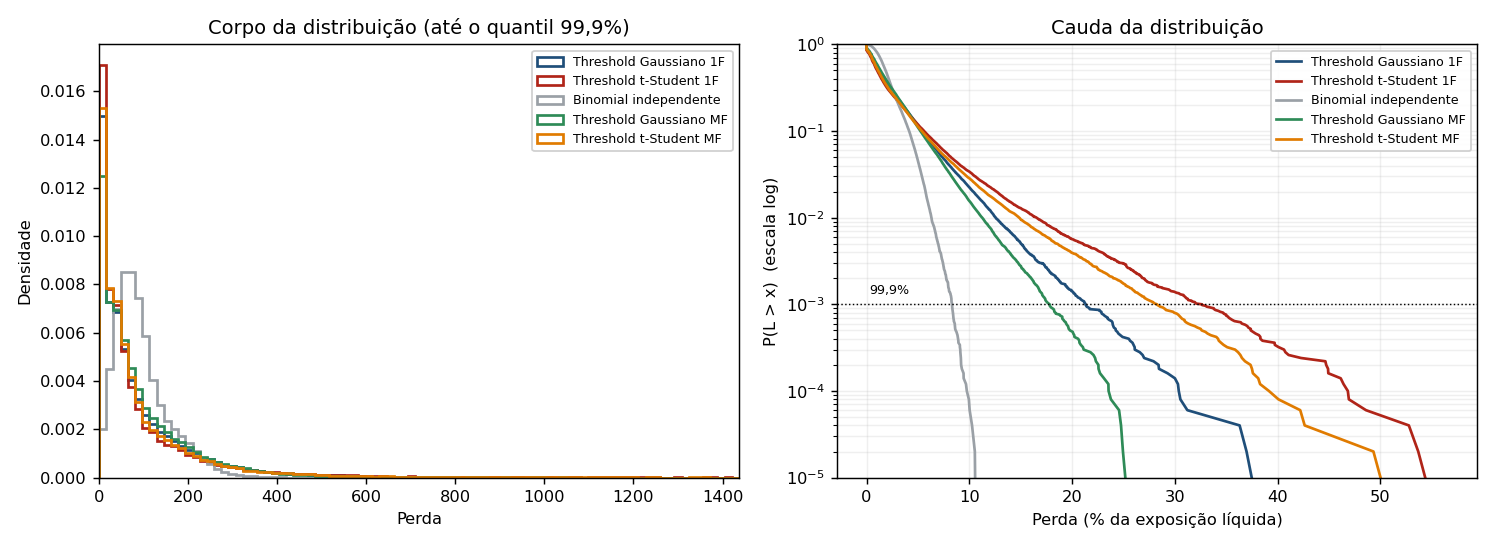
\includegraphics[width=\textwidth]{distribuicoes_perda.png}
\caption{Distribuição de perdas sob cinco modelos: corpo até o quantil de 99{,}9\% (esq.) e cauda em escala logarítmica (dir., linha pontilhada no nível de 99{,}90\%). No corpo, as distribuições são quase indistinguíveis; na cauda, separam-se por fator de até quatro vezes --- ilustrando por que a escolha da estrutura de dependência domina qualquer refinamento de PD individual. Note os pares um fator vs.\ multifatorial (azul/verde e vermelho/laranja): a estrutura setorial desloca a cauda para dentro em ambas as famílias.}
\label{fig:dist}
\end{figure}

\begin{figure}[htb]
\centering
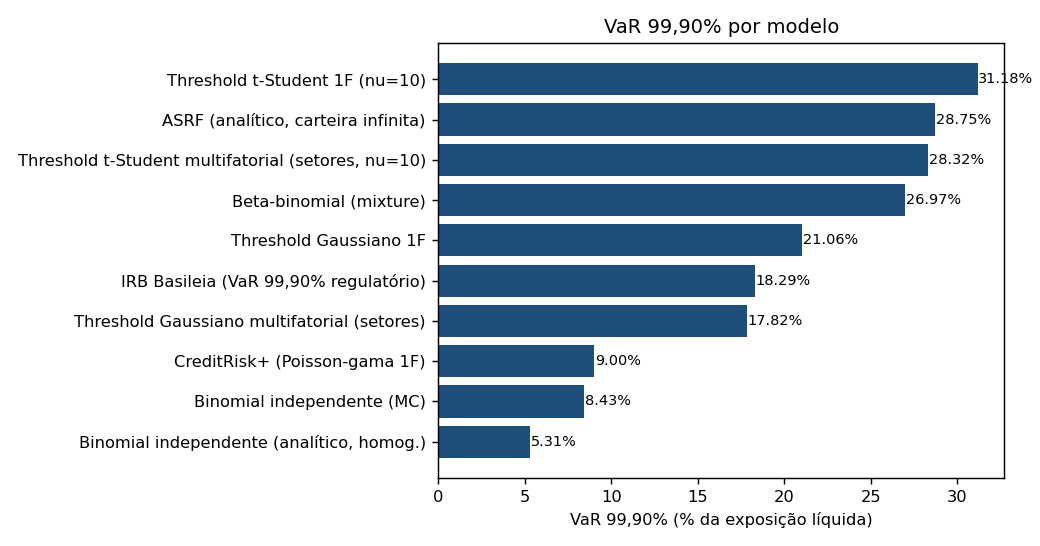
\includegraphics[width=0.8\textwidth]{var_por_modelo.png}
\caption{VaR 99{,}90\% por modelo, em percentual da exposição líquida.}
\label{fig:var}
\end{figure}

\subsection{Capital regulatório IRB}
\label{sec:ga-ex}

Aplicando \eqref{eq:irbK} contraparte a contraparte, o capital IRB da carteira é
\[
K^{*}=\sum_n c_n K_n = 710{,}1
\quad(16{,}13\%\ \text{da exposição líquida}),
\qquad
\mathrm{RWA} = 12{,}5\,K^{*} = 8\,876{,}7.
\]
O ajuste de granularidade adiciona $\mathrm{GA}=91{,}8$, elevando o requerimento a $801{,}9$ --- um acréscimo de 12{,}9\% sobre o capital IRB puro, coerente com os 89 nomes efetivos da carteira. Somado à perda esperada para permitir comparação com os VaRs totais dos modelos internos, o IRB$+$EL de $805{,}2$ (18{,}3\%) situa-se entre o \emph{threshold} gaussiano calibrado a $\rho_D=5\%$ e os modelos de cauda pesada. A leitura é direta: a correlação regulatória $\rho_B\in[12\%,24\%]$ é deliberadamente conservadora frente a calibrações internas típicas, mas a cópula gaussiana subjacente ao IRB não carrega dependência de cauda --- e o t-Student o ultrapassa com folga.

\subsection{Contribuições de risco}

\begin{table}[htb]
\centering\small
\caption{Dez maiores contribuições ao ES 99\% (decomposição MC, \emph{threshold} gaussiano, $S=10$).}
\label{tab:contrib}
\begin{tabular}{llrrrr}
\toprule
Contraparte & Rating & Exposição & PD & Contrib.\ ES & \% do ES \\
\midrule
CP0173 & CCC & 292{,}3 & 8{,}99\%  & 85{,}7 & 11{,}8\% \\
CP0156 & BB  & 217{,}1 & 2{,}34\%  & 40{,}7 & 5{,}6\% \\
CP0051 & C   & 47{,}5  & 24{,}41\% & 26{,}4 & 3{,}6\% \\
CP0092 & B   & 118{,}1 & 6{,}33\%  & 21{,}4 & 3{,}0\% \\
CP0078 & BBB & 266{,}8 & 0{,}63\%  & 21{,}2 & 2{,}9\% \\
CP0139 & BBB & 301{,}9 & 0{,}58\%  & 19{,}1 & 2{,}6\% \\
CP0103 & C   & 44{,}3  & 37{,}05\% & 19{,}1 & 2{,}6\% \\
CP0228 & B   & 87{,}3  & 5{,}38\%  & 16{,}1 & 2{,}2\% \\
CP0036 & B   & 109{,}2 & 3{,}67\%  & 15{,}9 & 2{,}2\% \\
CP0245 & C   & 101{,}4 & 15{,}55\% & 15{,}5 & 2{,}1\% \\
\bottomrule
\end{tabular}
\end{table}

A Tabela~\ref{tab:contrib} e a Figura~\ref{fig:contrib} revelam a anatomia da cauda. A contraparte CP0173 --- rating CCC com a segunda maior exposição da carteira --- responde sozinha por 11{,}8\% do ES 99\%: a combinação multiplicativa de PD alta com exposição alta que a alocação de capital deve penalizar no \emph{pricing}. Observe, porém, CP0078 e CP0139: ratings BBB, PDs abaixo de 65~pontos-base e, ainda assim, entre os seis maiores contribuintes --- puro efeito de tamanho (cerca de $300$ de exposição cada). A lição operacional é clara: a gestão de limites por rating, isoladamente, não controla a cauda; a métrica correta de concentração é a contribuição de risco, não a PD. Os dez nomes da tabela somam cerca de 39\% do ES total, contra 24\% da exposição --- a cauda é mais concentrada do que a própria carteira.

\begin{figure}[htb]
\centering
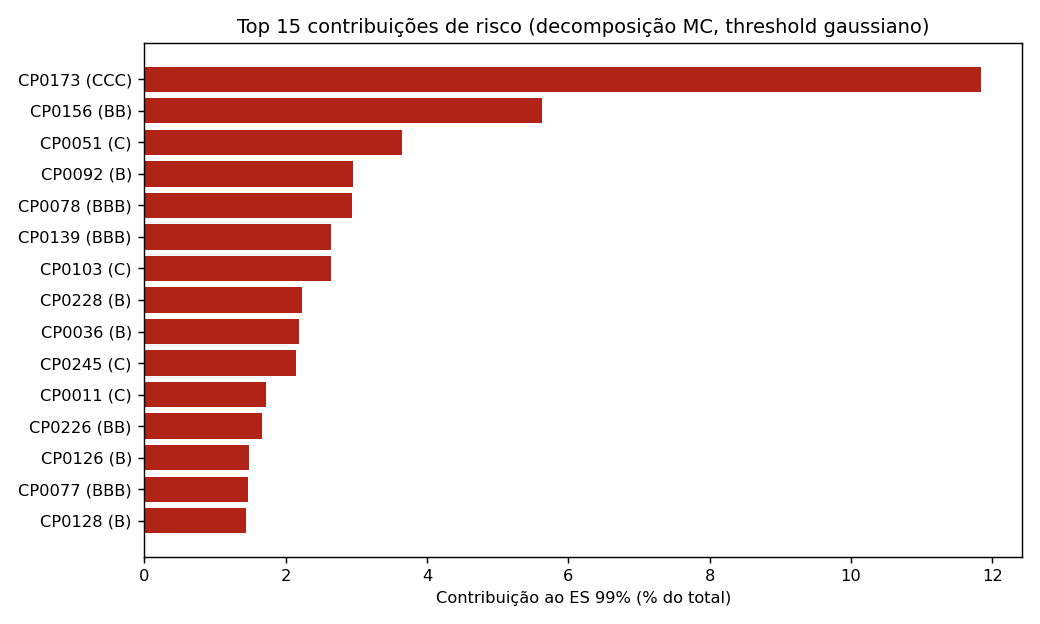
\includegraphics[width=0.85\textwidth]{contribuicoes_risco.png}
\caption{Quinze maiores contribuições ao ES 99\% (percentual do total).}
\label{fig:contrib}
\end{figure}

\subsection{Análise multifatorial setorial}
\label{sec:mf-ex}

A carteira de teste distribui-se em oito setores, com HHI setorial de $0{,}1364$ --- o equivalente a $7{,}3$ setores efetivos, uma diversificação setorial razoável, ainda que desigual: Energia detém $17{,}5\%$ da exposição líquida, enquanto Agro e Petroquímica, somados, não chegam a $13\%$. Com alvos de correlação de default de 8\% intra-setor e 3\% inter-setor, a calibração numérica via \eqref{eq:rhoD} produziu correlações de \emph{ativos} de $\rho_S=33{,}67\%$ e $\rho_G=17{,}02\%$ --- novamente a não linearidade em ação: dobrar ou triplicar a correlação de default exige quase o dobro da correlação de ativos.

\paragraph{O efeito diversificação.} A Tabela~\ref{tab:mf-comp} compara, nível a nível, o modelo de um fator (calibrado a $\rho_D=5\%$ uniforme) com o multifatorial. O padrão é consistente nas duas famílias: o multifatorial entrega medidas menores, e a redução \emph{cresce com o nível de confiança} --- de cerca de $-6\%$ no VaR 95\% a $-15\%$ no VaR 99{,}90\% do modelo gaussiano ($-19\%$ no ES). A razão é estrutural. No modelo de um fator, todos os $31\,125$ pares de contrapartes carregam a mesma correlação de default de 5\%; no multifatorial, apenas os pares \emph{dentro} de um mesmo setor (cerca de 13\% dos pares) operam ao alvo intra de 8\%, enquanto a grande maioria --- pares entre setores distintos --- opera a apenas 3\%.\footnote{A conta é verificável: com $N=250$, o total de pares é $\binom{250}{2}=\frac{250\times249}{2}=31\,125$. Os pares intra-setor são $\sum_s\binom{n_s}{2}$ sobre os oito setores; com os tamanhos da carteira de teste ($37$, $36$, $33$, $33$, $32$, $31$, $24$ e $24$ nomes), $666+630+528+528+496+465+276+276=3\,865$ pares, ou $12{,}4\%$ do total. A correlação de default média da carteira multifatorial fica, portanto, em torno de $0{,}124\times8\%+0{,}876\times3\%\approx3{,}6\%$ --- abaixo dos $5\%$ uniformes do modelo de um fator. Note que a fração intra-setor cresce quadraticamente com a concentração setorial (é o HHI setorial agindo sobre os pares): numa carteira concentrada em poucos setores, a média se aproximaria do alvo intra e a comparação poderia se inverter.} A correlação média da carteira cai, e cai justamente onde mais importa: nos cenários extremos, em que o fator global sozinho não basta para derrubar simultaneamente nomes de setores diferentes. A estrutura setorial, portanto, \emph{revela um benefício de diversificação que o fator único, ao aplicar 5\% indistintamente, não consegue distinguir} --- e a Figura~\ref{fig:mfcomp} mostra que o efeito se preserva, em menor grau ($-9\%$ no VaR 99{,}9\%), mesmo sob a dependência de cauda da variante t.

\begin{table}[htb]
\centering\small
\caption{Um fator vs.\ multifatorial setorial: VaR e ES por nível de confiança (unidades monetárias; variação percentual do multifatorial sobre o um fator).}
\label{tab:mf-comp}
\setlength{\tabcolsep}{4pt}
\begin{tabular}{lrrrrrrrr}
\toprule
& \multicolumn{4}{c}{Gaussiano} & \multicolumn{4}{c}{t-Student ($\nu=10$)}\\
\cmidrule(lr){2-5}\cmidrule(lr){6-9}
Nível $\alpha$ & 1 fator & Multif. & $\Delta$VaR & $\Delta$ES & 1 fator & Multif. & $\Delta$VaR & $\Delta$ES\\
\midrule
95\%     & 329{,}3   & 309{,}1 & $-6{,}1\%$  & $-10{,}9\%$ & 354{,}8   & 340{,}6   & $-4{,}0\%$ & $-6{,}9\%$\\
99\%     & 563{,}6   & 495{,}8 & $-12{,}0\%$ & $-14{,}7\%$ & 707{,}6   & 655{,}1   & $-7{,}4\%$ & $-9{,}9\%$\\
99{,}9\% & 927{,}1   & 784{,}7 & $-15{,}4\%$ & $-19{,}1\%$ & 1\,372{,}8 & 1\,246{,}9 & $-9{,}2\%$ & $-13{,}7\%$\\
99{,}97\%& 1\,129{,}9 & 959{,}6 & $-15{,}1\%$ & $-24{,}0\%$ & 1\,822{,}2 & 1\,592{,}0 & $-12{,}6\%$ & $-18{,}8\%$\\
\bottomrule
\end{tabular}
\end{table}

\begin{figure}[htb]
\centering
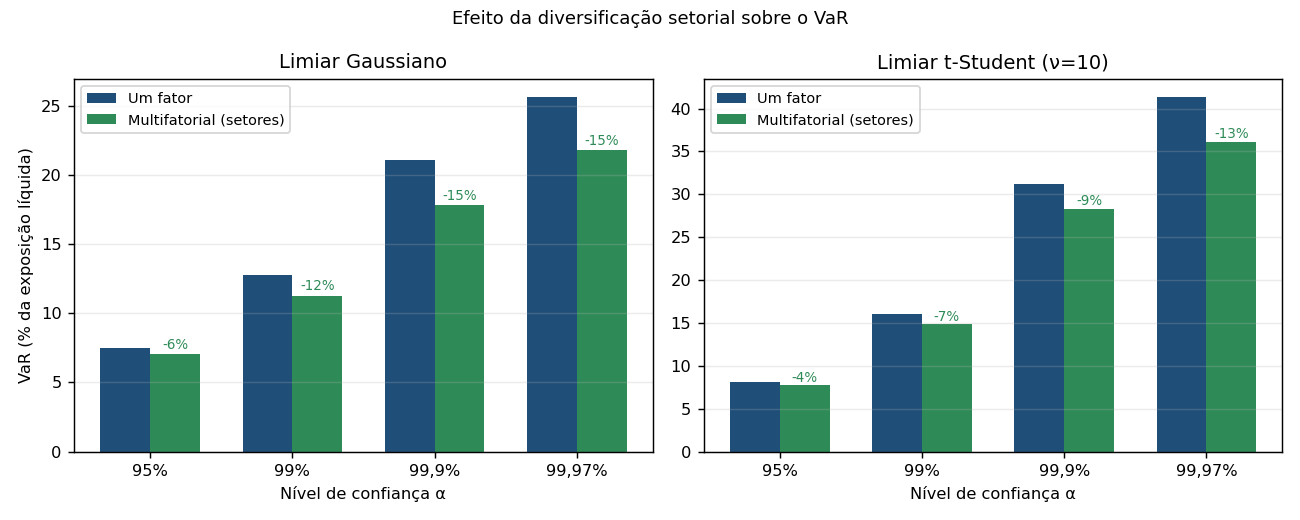
\includegraphics[width=0.95\textwidth]{comparacao_1f_mf.png}
\caption{VaR em percentual da exposição líquida, um fator vs.\ multifatorial, nas famílias gaussiana (esq.) e t-Student (dir.). Os rótulos indicam a variação percentual. O benefício de diversificação setorial cresce com o nível de confiança e persiste sob dependência de cauda.}
\label{fig:mfcomp}
\end{figure}

Há uma leitura de gestão importante aqui: o resultado \emph{não} diz que o multifatorial ``economiza capital'' por construção. Ele diz que, \emph{dada esta carteira bem espalhada em oito setores}, a premissa de correlação uniforme do fator único é conservadora. Numa carteira concentrada em poucos setores a comparação se inverteria --- os pares intra-setor a 8\% passariam a dominar --- e é exatamente essa sensibilidade à composição setorial que o modelo de um fator é incapaz de exibir.

\subsection{Contribuições por setor: exposição, provisão e cauda}
\label{sec:setores-ex}

\begin{table}[htb]
\centering\small
\caption{Decomposição setorial completa (\emph{threshold} gaussiano multifatorial; contribuições ao ES 99\%, $S=10$). Participações em percentual do total da carteira; razão = contribuição ao ES $\div$ exposição.}
\label{tab:setores}
\setlength{\tabcolsep}{4.5pt}
\begin{tabular}{lrrrrrrr}
\toprule
Setor & Nomes & Exposição & Exp.\ (\%) & EL & EL (\%) & ES (\%) & Razão \\
\midrule
Indústria    & 37 & 548{,}2 & 12{,}5 & 17{,}3 & 18{,}2 & 20{,}6 & 1{,}65 \\
Energia      & 24 & 772{,}1 & 17{,}5 & 13{,}4 & 14{,}1 & 20{,}5 & 1{,}17 \\
Serviços     & 36 & 556{,}3 & 12{,}6 & 23{,}8 & 25{,}1 & 15{,}8 & 1{,}25 \\
Varejo       & 33 & 652{,}8 & 14{,}8 & 9{,}1  & 9{,}6  & 12{,}6 & 0{,}85 \\
Construção   & 33 & 655{,}4 & 14{,}9 & 13{,}4 & 14{,}1 & 11{,}6 & 0{,}78 \\
Logística    & 31 & 646{,}1 & 14{,}7 & 5{,}6  & 5{,}9  & 9{,}5  & 0{,}65 \\
Agro         & 24 & 254{,}4 & 5{,}8  & 8{,}3  & 8{,}7  & 5{,}1  & 0{,}89 \\
Petroquímica & 32 & 317{,}3 & 7{,}2  & 4{,}2  & 4{,}4  & 4{,}3  & 0{,}60 \\
\midrule
Total & 250 & 4\,402{,}7 & 100 & 95{,}0 & 100 & 100 & 1{,}00 \\
\bottomrule
\end{tabular}
\end{table}

A Tabela~\ref{tab:setores} coloca lado a lado, para cada setor, as três participações que uma mesa de crédito precisa distinguir: na \emph{exposição} (quanto do balanço está ali), na \emph{perda esperada} (quanto da provisão o setor consome) e na \emph{cauda} (quanto do capital econômico o setor exige). A Figura~\ref{fig:setores} visualiza o contraste, e três perfis setoriais emergem com nitidez:

\paragraph{Setor de provisão: Serviços.} Com $12{,}6\%$ da exposição, Serviços consome $25{,}1\%$ da perda esperada da carteira --- o dobro da sua participação --- mas apenas $15{,}8\%$ da cauda. O setor abriga nomes de PD alta e porte moderado (a contraparte CP0051, rating~C com PD de $24{,}4\%$, é o caso extremo): inadimplência \emph{frequente}, que corrói resultado via provisão, mas cujo tamanho individual não tem força para produzir os cenários catastróficos que definem o capital.

\paragraph{Setor de cauda: Energia.} O espelho invertido. Com a \emph{maior} exposição setorial ($17{,}5\%$), Energia consome perda esperada \emph{abaixo} da sua participação ($14{,}1\%$) --- os nomes são majoritariamente de boa qualidade --- mas responde por $20{,}5\%$ do ES. O risco aqui não é a frequência de default, e sim o \emph{porte}: o setor concentra as maiores exposições individuais da carteira (CP0038 com $211$ e CP0039 com $97$ de EAD, por exemplo), e basta o cenário sistemático adverso alcançá-las para a perda saltar. É risco de capital, não de provisão.

\paragraph{Setor misto: Indústria.} O pior dos dois mundos, e o líder disparado da razão risco/exposição ($1{,}65$): com $12{,}5\%$ da exposição, o setor pesa $18{,}2\%$ na provisão \emph{e} $20{,}6\%$ na cauda. A explicação está na sua composição: Indústria combina o maior número de nomes (37) com a coexistência de exposições grandes e ratings fracos --- CP0173 (CCC, exposição $292{,}3$, o maior contribuinte individual da carteira) e CP0036 (B, $109{,}2$) pertencem ao setor. Concentração de porte \emph{e} de qualidade no mesmo lugar.

Na outra ponta, Logística e Petroquímica são os setores mais ``baratos'' em risco por unidade de exposição (razões de $0{,}65$ e $0{,}60$): carregam $14{,}7\%$ e $7{,}2\%$ do balanço a custo desproporcionalmente baixo de provisão e capital. Em linguagem de gestão de limites, são os setores com espaço para crescer; Indústria e Energia são os candidatos naturais a teto ou a exigência de garantias adicionais --- e a distinção entre os perfis importa para o \emph{tipo} de mitigação: em Serviços (provisão), a alavanca é \emph{pricing} e seleção; em Energia (cauda), é limite de concentração individual; em Indústria, ambas.

\begin{figure}[htb]
\centering
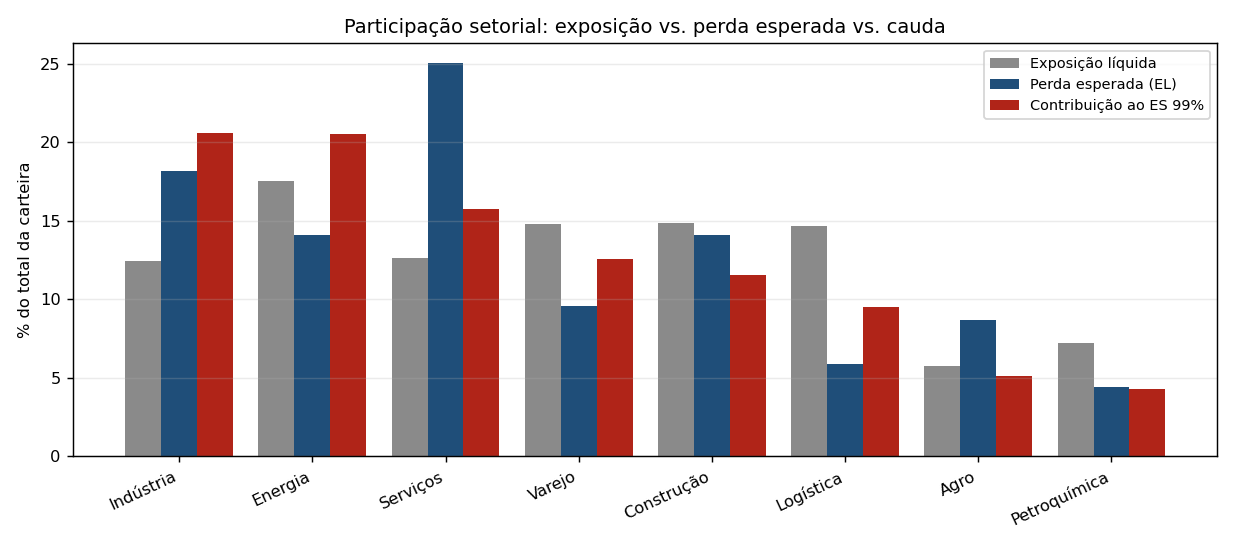
\includegraphics[width=0.95\textwidth]{setores_exposicao_el_es.png}
\caption{Participação de cada setor na exposição líquida, na perda esperada e na cauda (ES 99\%). A divergência entre as três barras de um mesmo setor revela o seu perfil de risco: EL acima da exposição indica frequência de default (provisão); ES acima da exposição indica concentração de porte (capital).}
\label{fig:setores}
\end{figure}

Por fim, vale registrar a consistência entre níveis de análise: os dez maiores contribuintes individuais da Tabela~\ref{tab:contrib} concentram-se exatamente nos três setores de razão mais alta --- CP0173, CP0036 e CP0228 em Indústria; CP0156 e CP0078 em Energia; CP0051 em Serviços ---, de modo que a leitura setorial e a leitura por nome contam a mesma história em granularidades diferentes. É essa coerência que permite usar as duas visões em conjunto: o setor define \emph{onde} apertar limites; a contribuição individual define \emph{quem}.

\subsection{Migração, ECL e capital multiperíodo}
\label{sec:mig-ex}

A matriz de exemplo (disponível em \texttt{templates/matriz\_migracao\_modelo.csv}) é diagonal-dominante, com massa concentrada nos estados vizinhos e coluna de default calibrada às PDs centrais dos oito graus da carteira de teste (de 3~pontos-base em AAA a 25\% em C). A Figura~\ref{fig:migracao} (painel esquerdo) mostra a estrutura a termo resultante: em escala logarítmica, as PDs acumuladas dos graus de investimento \emph{aceleram} com o horizonte --- um AAA praticamente não defaulta no ano 1, mas acumula risco à medida que a cadeia o deixa migrar para graus piores antes de defaultar ---, enquanto os graus especulativos, já próximos do default, crescem de forma quase linear. É o efeito de segunda ordem que nenhuma PD de 12 meses captura.

Aplicando \eqref{eq:ecl} com desconto de 10\%~a.a., o $\mathrm{ECL}^{12m}$ total é de $84{,}3$ --- próximo, mas não idêntico, à perda esperada de $95{,}0$ da Tabela~\ref{tab:resumo}: a diferença decorre de a matriz operar com a PD \emph{do grau}, enquanto a coluna \texttt{pd} da carteira carrega dispersão idiossincrática em torno do central de cada grau. O $\mathrm{ECL}^{\mathrm{life}}$ total é de $266{,}9$ --- \textbf{3{,}17 vezes o de 12 meses} ---, concentrado nos graus especulativos: B ($63{,}1$), CCC ($63{,}0$) e C ($59{,}0$) respondem juntos por $69\%$ do \emph{lifetime}, contra $75\%$ do 12 meses; os graus de investimento, irrelevantes no horizonte curto, passam a pesar via acumulação plurianual (painel direito da Figura~\ref{fig:migracao}). Na classificação de estágios, $20$ contrapartes apresentam deterioração de dois ou mais \emph{notches} frente à originação e migram a estágio~2; a provisão por estágio resultante é de $94{,}9$ --- $13\%$ acima do $\mathrm{ECL}^{12m}$ puro, o custo da regra de deterioração significativa nesta carteira.

\begin{figure}[htb]
\centering
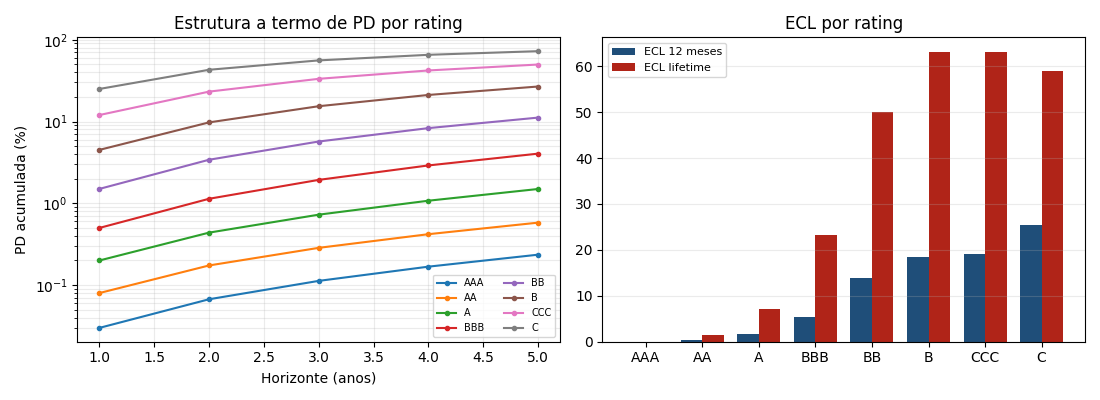
\includegraphics[width=0.95\textwidth]{migracao_ecl.png}
\caption{Esquerda: estrutura a termo de PD acumulada por rating (escala logarítmica), obtida das potências da matriz de transição. Direita: ECL 12 meses vs.\ \emph{lifetime} por grau de rating (desconto de 10\%~a.a.). A razão \emph{lifetime}/12m da carteira é de 3{,}17.}
\label{fig:migracao}
\end{figure}

Na simulação multiperíodo de $5$ anos ($M=100\,000$, blocos de $10\,000$, estrutura multifatorial setorial com os $\rho$ calibrados da Seção~\ref{sec:mf-ex}, desconto de 10\%~a.a.), a fração da carteira em default é estável em torno de $2{,}3\%$ ao ano --- coerente com a PD média ---, e a distribuição das perdas descontadas acumuladas entrega $\E[L]=354{,}1$, $\mathrm{UL}=186{,}7$, $\VaR_{99,9\%}=1\,223{,}4$ e $\ES_{99,9\%}=1\,340{,}5$. A comparação com o horizonte anual é instrutiva: o VaR 99{,}9\% de cinco anos ($27{,}8\%$ da exposição líquida) é apenas $56\%$ maior que o de um ano do mesmo modelo multifatorial ($784{,}7$), e não cinco vezes --- a diversificação \emph{temporal} (os cenários sistemáticos adversos não se repetem todos os anos) e o desconto comprimem a cauda acumulada. É precisamente o risco que o ajuste de maturidade do IRB aproxima por fórmula: aqui ele aparece medido por simulação, com a migração explícita.

\subsection{Da base analítica à carteira de modelagem: 300 mil contratos}
\label{sec:agg-ex}

Para exercitar a camada de agregação, uma base analítica sintética de $300\,000$ contratos (gerável no próprio aplicativo) combina varejo pulverizado com $300$ operações \emph{corporate} de porte duas ordens de grandeza maior, concentradas em poucos setores. A agregação com corte nas $200$ maiores exposições produz uma carteira de modelagem de \textbf{264 linhas} --- $200$ grandes exposições ($9{,}7\%$ da exposição) mais $64$ buckets GH$\times$setor --- em menos de um segundo, com \textbf{perda esperada preservada com diferença de $0{,}0000\%$} ($1\,180{,}8$ nas duas bases) e CV máximo de PD intra-bucket de $0{,}32$, dentro do padrão de homogeneidade. A suíte \emph{pooled} completa, com $M=100\,000$, roda em cerca de $25$ segundos.

\begin{table}[htb]
\centering\small
\caption{Medidas de risco da carteira agregada (300 mil contratos $\to$ 264 linhas; motor \emph{pooled}, $M=100\,000$; unidades monetárias). Exposição líquida total de $44\,959{,}3$.}
\label{tab:pooled}
\setlength{\tabcolsep}{4.5pt}
\begin{tabular}{lrrrrrr}
\toprule
Modelo & EL & UL & VaR$_{99\%}$ & ES$_{99\%}$ & VaR$_{99,9\%}$ & ES$_{99,9\%}$ \\
\midrule
Binomial independente (\emph{pooled}) & 1\,180 & 66 & 1\,382 & 1\,423 & 1\,477 & 1\,510 \\
Threshold Gaussiano 1F & 1\,178 & 1\,266 & 6\,119 & 7\,828 & 10\,002 & 11\,628 \\
Threshold t-Student 1F ($\nu=10$) & 1\,178 & 1\,628 & 7\,994 & 10\,982 & 15\,029 & 18\,298 \\
Threshold Gaussiano multifatorial & 1\,181 & 1\,092 & 5\,296 & 6\,487 & 7\,922 & 9\,226 \\
Threshold t-Student multifatorial ($\nu=10$) & 1\,188 & 1\,477 & 7\,371 & 9\,686 & 12\,775 & 15\,425 \\
ASRF (analítico) & 1\,181 & --- & 7\,829 & 10\,306 & 13\,540 & 16\,062 \\
\midrule
IRB Basileia ($K^{*}$, s/ EL) & --- & --- & --- & --- & 8\,234 \;(18{,}3\%) & --- \\
\bottomrule
\end{tabular}
\end{table}

A Tabela~\ref{tab:pooled} tem duas leituras que a carteira granular de 250 nomes não podia oferecer. A primeira é a \emph{morte do risco idiossincrático}: o modelo binomial independente, que na carteira pequena ainda produzia UL relevante, colapsa aqui para UL de $66$ contra $1\,266$ do \emph{threshold} gaussiano --- vinte vezes menos. Com $300$ mil contratos, a lei dos grandes números elimina praticamente toda a variabilidade não sistemática, e a distribuição de perdas passa a ser, para todos os efeitos, uma função do ciclo: é a materialização empírica da premissa assintótica do ASRF, e a razão pela qual capital de carteiras pulverizadas é inteiramente uma discussão sobre correlação com o fator sistemático. A segunda leitura é a coerência do ajuste de granularidade: o GA despenca para $8{,}7$ --- ante $91{,}8$ na carteira de 250 nomes --- porque os pools têm granularidade interna quase perfeita ($C_g^2/n_g\to 0$) e as $200$ grandes exposições respondem por apenas $9{,}7\%$ do livro. O benefício de diversificação setorial segue presente e material: o multifatorial reduz o VaR 99{,}9\% gaussiano em $21\%$ ($10\,002\to7\,922$).

\begin{figure}[htb]
\centering
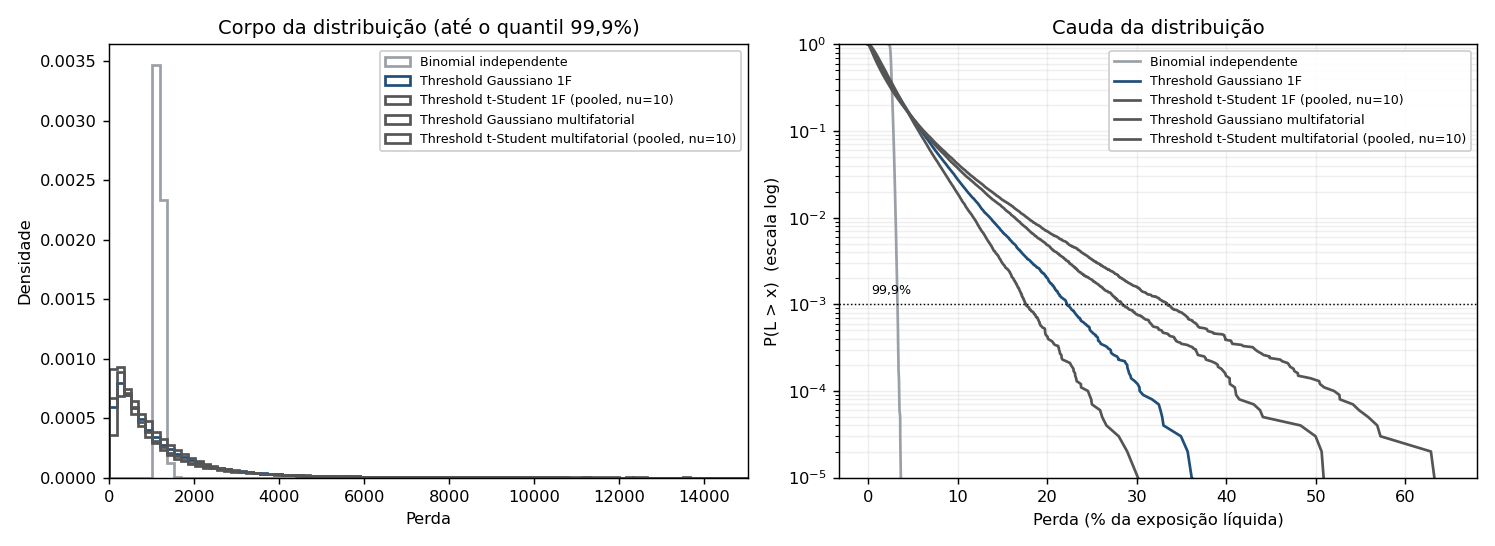
\includegraphics[width=\textwidth]{pooled_distribuicoes.png}
\caption{Distribuição de perdas da carteira agregada (300 mil contratos, motor \emph{pooled}). A curva do modelo independente, quase degenerada em torno da EL, ilustra a eliminação do risco idiossincrático pela lei dos grandes números; toda a dispersão remanescente nos demais modelos é risco sistemático.}
\label{fig:pooled}
\end{figure}

Uma nota de interpretação: os índices de concentração do resumo (HHI, top-10) passam a se referir às \emph{linhas} da carteira agregada, não aos contratos --- a concentração verdadeira de nomes está preservada nas grandes exposições individuais e, no capital, via o termo $C_g^2/n_g$ do GA. O módulo de migração opera integralmente sobre a carteira agregada. O ECL por bucket é exato --- a matriz trabalha com a PD do grau, que é o próprio critério de formação do GH --- e totaliza $1\,029{,}8$ em 12 meses contra $3\,383{,}1$ \emph{lifetime} (razão de $3{,}29$, desconto de 10\%~a.a.). E o multiperíodo roda no modo \emph{pooled} da equação \eqref{eq:mig-pooled}: em cinco anos, com a estrutura multifatorial setorial, a perda descontada acumulada tem $\E[L]=4\,488{,}4$ --- que reproduz a esperança analítica da matriz descontada ($4\,497{,}4$) com desvio de $-0{,}2\%$, a validação de sanidade do motor --- e $\VaR_{99,9\%}=13\,221{,}5$ ($29{,}4\%$ da exposição líquida), cerca de $1{,}7$ vez o VaR de um ano do mesmo modelo: novamente a diversificação temporal comprimindo a cauda acumulada. A fração de contratos em default cresce de $2{,}53\%$ para $2{,}70\%$ ao ano ao longo do horizonte --- a deriva de migração da carteira, invisível a qualquer análise de 12 meses.

\section{Limitações e extensões}

A versão atual carrega quatro premissas simplificadoras, cada qual com extensão natural já mapeada na própria biblioteca de Bolder.

A LGD é determinística. A generalização estocástica --- severidade sorteada de uma distribuição beta, correlacionada ou não com o ciclo --- está implementada na rotina \texttt{crPlusOneFactorLGD} e seria o primeiro refinamento em aplicação prudencial, dado o papel conhecido da volatilidade de LGD nas caudas.

A correlação intra-setor é uniforme: todos os setores compartilham o mesmo $\rho_S$. Cargas setoriais heterogêneas --- setores cíclicos mais correlacionados que defensivos --- são a generalização direta, na estrutura de \texttt{buildAssetCorrelationMatrix} e \texttt{getY2r}.

O Monte Carlo é simples. Para quantis muito extremos (99{,}97\% e além) ou carteiras grandes, o capítulo~8 do livro fornece \emph{importance sampling} com deslocamento ótimo de média, capaz de estimar a cauda com uma fração das simulações; as rotinas correspondentes já acompanham a biblioteca.

Na camada de agregação, os buckets são tratados como internamente homogêneos (mesma PD e severidade média por contrato); dispersões intra-bucket relevantes pedem GHs mais finos, e o relatório de CV de PD existe para vigiar essa premissa. A matriz de transição é insumo do usuário, e o ajuste de granularidade usa os parâmetros de volatilidade setorial de referência do livro. As extensões naturais são, respectivamente: estimar a matriz a partir do histórico de ratings da própria carteira, pelos métodos de coorte e de \emph{hazard rate} com intervalos de confiança por \emph{bootstrap} (módulo \texttt{markovChain}); estimar a volatilidade setorial a partir dos dados; e evoluir o módulo de migração para o modo \emph{mark-to-market} à la CreditMetrics, que reutilizaria a mesma escada de limiares da Seção~\ref{sec:migracao} com revalorização por banda de destino.

\section*{Referências}

\begin{itemize}\setlength\itemsep{1pt}
\item[] Bolder, D.~J. (2018). \emph{Credit-Risk Modelling: Theoretical Foundations, Diagnostic Tools, Practical Examples, and Numerical Recipes in Python}. Springer. [Referencial teórico e bibliotecas numéricas, \texttt{github.com/djbolder/credit-risk-modelling}, GPL-3.0.]
\item[] Basel Committee on Banking Supervision (2005). \emph{An Explanatory Note on the Basel II IRB Risk Weight Functions}. BIS.
\item[] Gordy, M.~B. (2003). A risk-factor model foundation for ratings-based bank capital rules. \emph{Journal of Financial Intermediation}, 12(3), 199--232.
\item[] Gordy, M.~B.; Lütkebohmert, E. (2013). Granularity adjustment for regulatory capital assessment. \emph{International Journal of Central Banking}, 9(3), 33--71.
\item[] Vasicek, O. (2002). The distribution of loan portfolio value. \emph{Risk}, 15(12), 160--162.
\end{itemize}

\end{document}
